\documentclass[10pt, varwidth]{standalone}

%
% compile using: pdflatex -shell-escape reu_paper.tex
%

\usepackage{tikz}
\usetikzlibrary{calc}
\usetikzlibrary{shapes,arrows}

\usepackage{pgfplots}

\usepackage{caption}
\usepackage{amsmath}
\usepackage{graphics}
\usepackage{graphicx}
\usepackage{multicol}
\usepackage{amsfonts}
\usepackage{algorithm}
\usepackage{algorithmic}
\usepackage{mdwlist}
\usepackage{mathtools}
\usepackage{url}

\date{}

\begin{document}
\vspace{-3cm}

	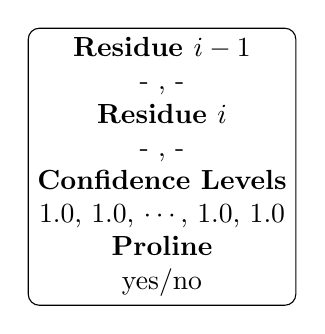
\begin{tikzpicture}

		% tiles
		\node[align=center, rounded corners, draw] {\textbf{Residue $i-1$}\\
		- , -\\
		\textbf{Residue $i$}\\
		- , -\\
		\textbf{Confidence Levels}\\
		1.0, 1.0, $\cdots$, 1.0, 1.0\\
		\textbf{Proline}\\
		yes/no};

	\end{tikzpicture}
\end{document}